\section{Experiment 10H-B: observer-mechanism audit}
\label{sec:experiment10hb}

\paragraph{Question and preregistered logic.}
Experiment 10H-A established that normalized tire forces and sideslip are
observable, but a fleet-global observer caused a large closed-loop tail loss.
Experiment 10H-B separates three possible causes: sensor bias, mismatch within
a compatible vehicle class, and mismatch caused by pooling incompatible
classes. The key question is whether class-compatible observer sharing removes
enough of the GlobalKF loss to justify a clustered-federated observer stage.

The fleet, ten confirmation seeds (511--520), H03 Global LQI controller,
measurement covariance, observer process covariance, maneuvers, and all
controller parameters are frozen from Experiments 10H and 10H-A. No tuning is
performed in 10H-B. The predefined gates require the oracle-class observer to
recover at least 25\% of the GlobalKF-to-ExactKF tracking gap, remain within
10\% of ExactKF on average, outperform GlobalKF at all four mean/worst and
broadband/transient endpoints, and keep every trajectory finite.

\paragraph{Factorial observer comparison.}
The same measurements $y=[r,a_y,\delta_a]^\top$ are supplied to three
scheduled Kalman observers:
\begin{itemize}
  \item ExactKF uses the exact client matrices and isolates the observer and
        measurement interface;
  \item OracleClassKF uses matrices averaged only within the known compact,
        sport, or SUV class and isolates within-class mismatch;
  \item GlobalKF averages all classes and adds cross-class mismatch.
\end{itemize}
Each observer is tested with measurement noise only and with the same noise
plus trajectory-constant sensor biases. Common random numbers are used for
every paired observer comparison. FullState is retained as a reference, but
the ExactKF--FullState contrast must be interpreted as the net effect of
filtered output feedback, not as a pure additive noise effect: filtering also
changes the effective behavior of the aggressive full-state controller.

\begin{table}[htbp]
\centering
\caption{Experiment 10H-B mean yaw-rate tracking RMSE [deg/s].}
\label{tab:experiment10hb-performance}
\begin{tabular}{llrrr}
\toprule
Maneuver & Measurement condition & ExactKF & OracleClassKF & GlobalKF\\
\midrule
Broadband & Noise only       & 0.14535 & 0.14646 & 0.16642\\
Broadband & Noise plus bias  & 0.15335 & 0.15441 & 0.17402\\
Transient & Noise only       & 0.13121 & 0.13291 & 0.14880\\
Transient & Noise plus bias  & 0.13931 & 0.14094 & 0.15647\\
\bottomrule
\end{tabular}
\end{table}

\paragraph{Mechanism attribution.}
Table~\ref{tab:experiment10hb-mechanisms} reports paired percentage changes.
Bias is material but is not the main explanation for GlobalKF's poor tail.
Within a true class, residual model mismatch costs only 0.69--2.42\%. Moving
from the class observer to one fleet-global observer adds 11.02--33.79\%.
Thus the damaging mismatch is predominantly between classes, not between
clients within a class.

\begin{table}[htbp]
\centering
\caption{Incremental observer mechanisms. Positive values denote worse
tracking than the preceding baseline.}
\label{tab:experiment10hb-mechanisms}
\begin{tabular}{llrrr}
\toprule
Maneuver & Endpoint & Sensor bias & Within class & Cross class\\
\midrule
Broadband & Mean  & 5.50\% & 0.69\% & 12.70\%\\
Broadband & Worst & 6.32\% & 2.42\% & 33.79\%\\
Transient & Mean  & 6.18\% & 1.16\% & 11.02\%\\
Transient & Worst & 11.29\% & 2.13\% & 28.97\%\\
\bottomrule
\end{tabular}
\end{table}

\begin{table}[htbp]
\centering
\caption{OracleClassKF recovery of the GlobalKF-to-ExactKF gap. Intervals are
paired seed-bootstrap 95\% intervals.}
\label{tab:experiment10hb-recovery}
\begin{tabular}{llrr}
\toprule
Maneuver & Endpoint & Gap recovery & 95\% CI\\
\midrule
Broadband & Mean  & 94.87\% & [94.36,95.40]\%\\
Broadband & Worst & 93.83\% & [90.74,96.77]\%\\
Transient & Mean  & 90.52\% & [89.19,92.01]\%\\
Transient & Worst & 94.34\% & [90.48,98.37]\%\\
\bottomrule
\end{tabular}
\end{table}

Every output-feedback trajectory is finite and all predefined gates pass.

\begin{figure}[htbp]
\centering
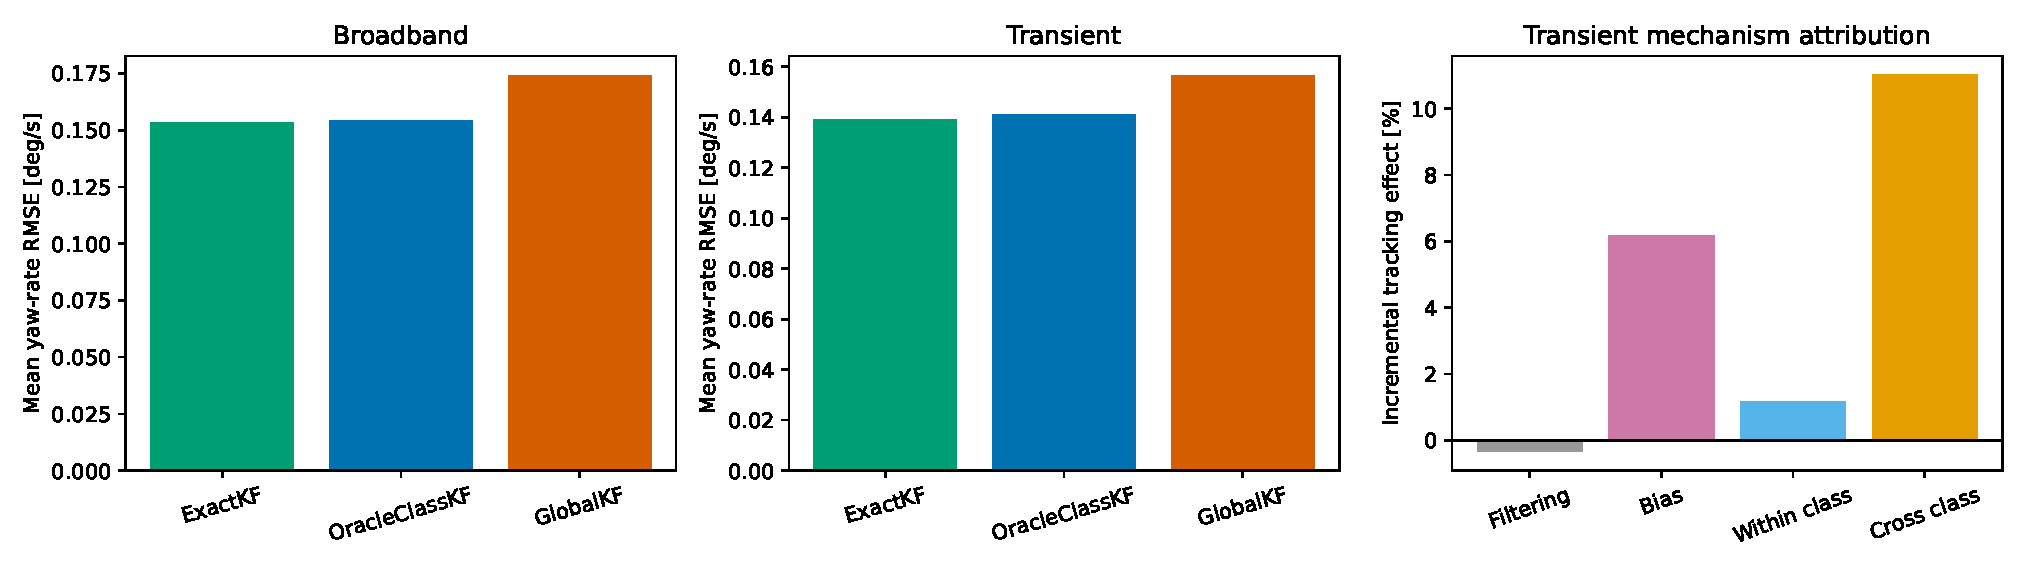
\includegraphics[width=0.98\linewidth]{../results/figures/experiment_10hb_observer_mechanism.pdf}
\caption{Biased output-feedback performance and incremental mechanism
attribution in Experiment 10H-B.}
\label{fig:experiment10hb}
\end{figure}

\paragraph{Interpretation and decision.}
This audit reverses the broad conclusion one might draw from 10H-A. Shared
observers are not intrinsically unsuitable. A single observer pooled across
incompatible vehicle classes is unsuitable; a class-compatible shared
observer is nearly as effective as a client-exact observer. This identifies a
specific and control-relevant role for clustered FL: learn compatible groups
and aggregate their higher-order LPV observer models without centralizing
client trajectories. Sensor-bias estimation remains a separate engineering
improvement and should not be credited to FL.

The result is still oracle evidence because the class labels are known. The
next experiment should replace those labels by learned assignments using only
federated model updates or privacy-preserving update summaries, freeze the
number of groups from data, and test whether the learned clustered observer
retains the oracle gap recovery on untouched fleets. A failure there would
limit the claim to known-class sharing; a success would connect complementary
coverage, clustered FL, state estimation, and LQI control in one chain.

\paragraph{Reproducibility.}
Configuration and implementation are in
\path{code/config/experiment_10hb.json} and
\path{code/experiments/experiment_10hb_observer_mechanism.py}. Client-level
records, seed summaries, paired mechanism effects, gap-recovery intervals,
gate decisions, and provenance hashes are stored under \path{results}.
